%!TEX root = main.tex

\section{Analysis of Voice Recognition Flow}

\subsection{Analysis Framework}

\begin{figure}[th]
\centering
	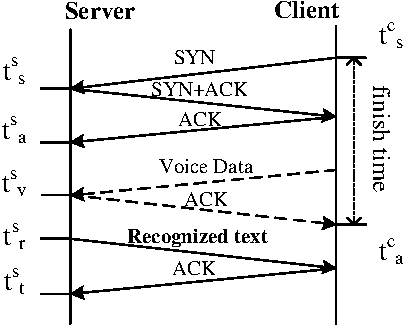
\includegraphics[scale=0.7]{voice_flow_rtt}
\caption{Time-line in voice recognition flow.}
\label{fig:voice_flow_rtt}
\end{figure}

Figure~\ref{fig:voice_flow_rtt} shows the time-line in voice recognition flow. From client side, the finish time is from that client initiates the connection to that client receives all acknowledgments of the voice data, \ie $t^c_a - t^c_s$. From server side, finish time is approximated as $(t^s_v - t^s_s) + (t^s_t - t^s_r)$, where $t^s_v$ is the time that server receives all voice data. As mentioned above, at most 3 RTT's could be measured from server side in voice recognition, including $t^s_a - t^s_s$ and $t^s_t - t^s_r$ in the figure, as well as the RTT when server terminates connection (not shown in the figure).

\begin{figure*}[th]
\centering
	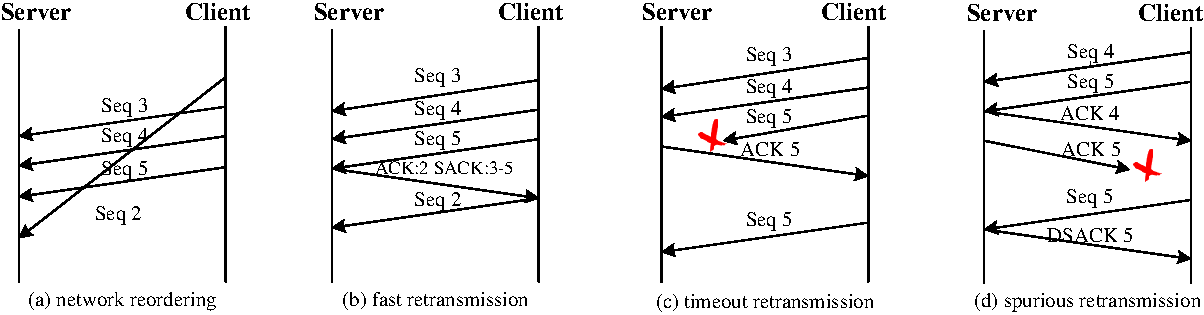
\includegraphics[scale=0.7]{voice_flow_estimate_retrans}
\caption{Server could not distinguish network congestion event when receiving voice data.}
\label{fig:voice_flow_estimate_retrans}
\end{figure*}

RTT is ambiguous when the corresponding segment is retransmitted. To investigate the impact of RTT on finish time, we use the following strategy to determine the minimal RTT. If there is no retransmission of SYN packet, $t^s_a - t^s_s$ is used as the RTT of the flow. Otherwise, the RTT when server terminates the connection is used, if the FIN packet is not retransmitted. When both of the two RTT's above are ambiguous, $t^s_t - t^s_r$ is exploited. We have verified in the web search dataset that $t^s_a - t^s_s$ is the minimal RTT in more than 60\% of flows, and is less than 2 times of the minimal RTT in 95\% of flows. Thus it is reasonable to assume that the measured RTT from server side could represent the minimal RTT from client side in voice recognition.

Besides the estimation of RTT, server could not distinguish network congestion event when receiving data from client, which is exemplified in Figure~\ref{fig:voice_flow_estimate_retrans}. In Figure~\ref{fig:voice_flow_estimate_retrans}(a), there are packets reordered by network, which has the same appearance at server side as that with fast retransmission in Figure~\ref{fig:voice_flow_estimate_retrans}(b). Actually, there is not packet loss in the former case, while there is in the latter case. In Figure~\ref{fig:voice_flow_estimate_retrans}(c), client retransmitted segment 5 when RTO timer is triggered. Server could not detect that the packet is retransmitted or reordered, but only sense that the packet is delayed for a longer time, compared to other packets. In fact, server could only detect unnecessary retransmission when receiving the same data packet twice, and notifies the spurious retransmission to client via Duplicate SACK~\cite{rfc3078}, which is shown in Figure~\ref{fig:voice_flow_estimate_retrans}(d).

To depict network congestion, we need two more metrics besides RTT: packet reordering and timeout retransmission. We use the number of disordered packets to represent the severity of packet reordering. The number of disordered packets is defined as follows. In receiving sequence $S_1, S_3, S_4, S_2$, the packet $S_2$ is disordered, thus the number of disordered packets is 1. In the following, we will take packet reordering as an indication of network congestion and study the impact of network congestion on finish time. Timeout retransmission means more severe network congestion. As illustrated in the figure above, timeout retransmission could not directly identified by server when receiving voice data. We rely on the following estimation to detect timeout retransmission. For each packet, there is an estimated arrival time, calculated according to that of preceding and subsequent packets. If the gap between actual arrival time and the estimated arrival time is larger than $max(200ms, 3 RTT)$, it is identified as a RTO. In the following, we also investigate the impact of timeout retransmission on finish time in voice recognition.

\subsection{Causal Analysis of Finish Time}

In this section, we first describe the poor performance that voice recognition flows experience, which inspires us to understand how the network condition leads to such results.

\begin{table}[th]
\centering
\renewcommand{\arraystretch}{1.2}
\caption{Percentage of abnormal flows in different ISP's.}
\label{tab:voice_stats}
\begin{tabular}{l|c|c|c}
	\toprule
	 & CT & CU & CM \\
	\midrule
	% packet reordering & 2.3\% & 3.1\% & 4.9\% \\
	% \hline
	SYN retransmission & 2.1\% & 1.7\% & 4.5\% \\
	\hline
	timeout retransmission & 5.3\% & 4.9\% & 4.9\% \\
	\hline
	incomplete transmission & 0.2\% & 0.3\% & 2.4\% \\
	\bottomrule
\end{tabular}
\end{table}

Table~\ref{tab:voice_stats} shows the percentage of abnormal flows in each ISP. A flow is abnormal if it encounters timeout retransmission, or incomplete transmission. The timeout retransmission could happen during 3-way handshake, or in data transmission. A flow is incomplete if the flow is terminated, yet there are unacknowledged data packets, which could happen after several timeout retransmissions.

In the table, about $1.7\sim4.5$ percentage of flows encounter RTO when establishing connections, which is named SYN retransmission. SYN retransmission greatly harms the finish time due to two reasons. First, the time for establishing connections is irrelevant to data transmission, yet occupies huge portion of flow latency. Second, the initial RTO is set to 1 second \cite{rfc62982011computing} as there is no RTT measured. When the SYN packet is dropped, it has to wait at least 1 second for retransmission, which is another great penalty to the finish time.

About 5\% of flows experience timeout retransmission when transferring data packet. In voice recognition flows, timeout retransmission has a devastating effect on the performance, and is easy to be activated. Most of voice recognition flows have no more than 6 data packets. When one of the last three packets is dropped, sender has to rely on RTO for retransmission. Compared to the ideal data transmission time, RTO is often tens of, or even hundreds of times higher \cite{flach2013reducing}.

Table~\ref{tab:voice_stats} also shows the percentage of incomplete flows. An extreme case is that the percentage of incomplete flows is 2.4\%. The flow is terminated before finishing data transmission, either by TCP stack after several RTO's, or by consumer after waiting for a intolerably long time. The non-negligible ratio of incomplete flows indicates poor user-perceived performance, which motivates us to understand the reasons behind.

\begin{table}[th]
\caption{The average RTT and number of disordered packets for each access type.}
\label{tab:voice_access_type_stats}
\centering
\renewcommand{\arraystretch}{1.2}
\begin{tabular}{l|l|l|l|l|l|l}
	\toprule
	& \multicolumn{3}{c|}{ RTT(s) } & \multicolumn{3}{c}{ \#(disordered packets) } \\
	\midrule
	ISP & CT & CU & CM & CT & CU & CM \\
	\midrule
	wifi & 0.1 & 0.088 & 0.198 & 0.026 & 0.034 & 0.056 \\
	\hline
	2G & 0.062 & 0.029 & 0.07 & 0.079 & 0.046 & 0.057 \\
	\hline
	3G & 0.039 & 0.025 & 0.052 & 0.078 & 0.038 & 0.069 \\
	\hline
	4G & - & - & 0.05 & - & - & 0.01 \\
	\bottomrule
\end{tabular}
\end{table}

Table~\ref{tab:voice_access_type_stats} shows the average RTT and number of disordered packets for each access type. From the table, we could see that flows in different access types experience different network conditions. For example, compared to flows in cellular network (2G/3G/4G), the flows in WiFi network have larger RTT values, yet fewer disordered packets. Even for the same access type, different ISP's have quite different network performance. Among the three ISP's, CM WiFi network has the largest RTT value, and most disordered packets. 

First, we need to exclude the impact of flow size on finish time in voice recognition. We use Pearson correlation coefficient to inspect their relationship in the three ISP's. The absolute values of the coefficients in three ISP's are less than 0.003, which demonstrates the finish time is completely irrelevant to the flow size. As most of flows contain no more than 6 data packets, the data could be packed within the initial congestion window from client side.

% TODO explain the reason why flows in CU experience such a high transmission time.
\begin{figure}[!htbp]
\centering
	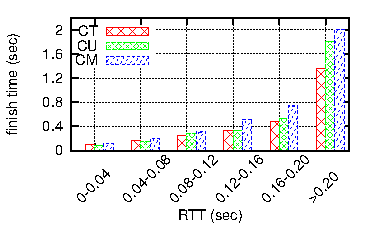
\includegraphics[width=3in]{voice_rtt}
\caption{The finish time under various RTT's in voice recognition.}
\label{fig:voice_rtt}
\end{figure}

Next, we study the impact of RTT on the finish time in voice recognition. We group the flows into different bins by their RTT's, with 0.04 second intervals. Figure~\ref{fig:voice_rtt} plots the average finish time of flows in each bin. From the figure, as the RTT value becomes larger, the finish time increases correspondingly. When the RTT value is less than 0.20 second, finish time has a roughly linear relationship with RTT. In fact, the correlation coefficients between the mean value of finish time in each bin and the index are more than 0.81 in all three ISP's. In the figure, the ratio of average finish time to the RTT value falls in the interval $[2, 4]$, except that when RTT value is larger than 0.2 second. When the RTT value is larger than 0.2 second (corresponding to 8\% of flows), the average finish time is more than 1.3 second. The reason is as follows. Larger RTT indicates that the packets are buffered in the network for longer time, which is also a signal of network congestion, as used in TCP Vegas\cite{brakmo1995tcp} and FastTCP\cite{wei2006fast}. Thus when flow experiences large RTT, it is likely that the flow is traversing congested network, and may encounter packet loss, takes at least one RTT for recovery.

\begin{table}[th]
\caption{Finish time under different RTT values using QED.}
\label{tab:voice_qed_rtt}
\centering
\renewcommand{\arraystretch}{1.2}
\begin{tabular}{l|m{.35in}|m{.35in}|m{.35in}}
	\toprule
	RTT bin (s) & CT & CU & CM \\
	\midrule
	$[$ 0.04, 0.08 ) & 1.50 & 1.60 & 1.52 \\
	\hline
	$[$ 0.08, 0.12 ) & 1.83 & 2.69 & 1.97 \\
	\hline
	$[$ 0.12, 0.16 ) & 2.76 & 3.22 & 3.23 \\
	\hline
	$[$ 0.16, 0.20 ) & 3.72 & 5.40 & 8.06 \\
	\hline
	$[$ 0.20, $\infty$ ) & 13.2 & 25.6 & 29.2 \\
	\bottomrule
\end{tabular}
\end{table}

We take the mean finish time in the bin $[$ 0, 0.04 ) as the baselines in three ISP, and use QED to investigate the performance degradation by larger RTT. The ratio of average finish time 
to baseline in each RTT bin is shown in Table~\ref{tab:voice_qed_rtt}. From the table, larger RTT leads to longer finish time, which confirms the result in Figure~\ref{fig:voice_rtt}. Similarly, when RTT value is less than 0.2 second, the finish time is proportional to the RTT value. When RTT is larger than 0.2 second, finish time grows rapidly. Larger RTT value indicates network congestion. When there is packet loss, client may rely on RTO for recovery, due to insufficient number of SACK's.

\begin{figure}[th]
\centering
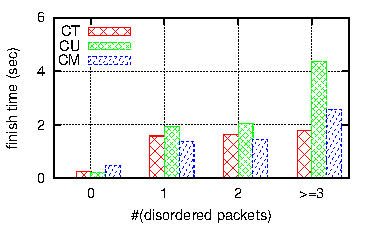
\includegraphics[width=3in]{voice_reorder}
\caption{The finish time under different number of disordered packets in voice recognition.}
\label{fig:voice_reorder}
\end{figure}

Figure~\ref{fig:voice_reorder} shows the average finish time under different number of disordered packets. From the figure, in all three ISP's, when there are disordered packets, flows experience significant performance degradation.

Even when there is only 1 disordered packet, the average finish time is 2$\sim$8 times higher than that of flows without disordered packet. This could be explained as follows. If server receives packets which are not successive, it feeds back to the client with SACK. When receiving SACK, client does not retransmit the packet in the hole (\ie the disordered packet) immediately, until client receives 3 SACK's or ACK of that packet, or retransmission timer is triggered. If the packet is dropped, client needs to wait at least one RTT to retransmit the packet. If there are not sufficient number of SACK's, client has to rely on timeout retransmission (RTO). The RTO timer, as an estimate of the RTT and variation in RTT, is usually highly conservative, which is set to tens of, or even hundreds of RTT. Especially in CU, when flows have more than 2 disordered packets, the average finish time is 20 times higher than that of flows without packet reordering.

\begin{table}[th]
\caption{Finish time under different number of disordered packets.}
\label{tab:voice_qed_reorder}
\centering
\renewcommand{\arraystretch}{1.2}
\begin{tabular}{c|c|c|c}
	\toprule
	\#(disordered packet) & CT & CU & CM \\
	\midrule
	1 & 1.05 & 1.11 & 1.32 \\
	\hline
	$\ge$ 2 & 1.59 & 2.17 & 1.38 \\
	\bottomrule
\end{tabular}
\end{table}

Table~\ref{tab:voice_qed_reorder} shows the ratio of finish time under different number of packets to the baseline (\ie finish time of flows with no disordered packet), using QED. From the table, as the number of disordered packets increases, the finish time increases slightly. Together with the results in Figure~\ref{fig:voice_reorder}, packet reordering has limited impact on finish time, unless the disordered packet is retransmitted by RTO.

\begin{figure}[th]
\centering
	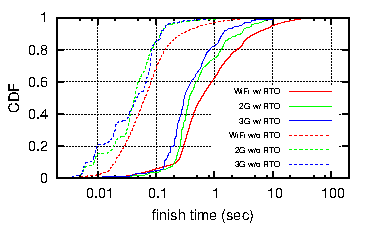
\includegraphics[width=\linewidth]{voice_timeout}
\caption{CDF of finish time of flows with and without RTO.}
\label{fig:voice_rto}
\end{figure}

Figure~\ref{fig:voice_rto} shows the CDF of finish time of flows with and without RTO. Note that the x-axis in the figure is plotted in log scale. From the figure, there is a remarkable performance gap between flows with RTO and that without RTO. The gap could be ten times for the median value. If there is no RTO, client needs 2-7 RTT's to transmit the voice data (1 RTT for each packet in worst case). However, if a packet is dropped and there are no sufficient subsequent data packets, the RTO will occupy most of the finish time, which could be tens of, or hundreds of RTT's.

\subsection{Summary of Voice Recognition Analysis}

In this section, we have analyzed the factors that impact on finish time in voice recognition flows. As the flow size is small (less than 7 data packets), the voice data could be fitted into the initial congestion window from client side, thus the finish time of flow is irrelevant to the size of the flow.

Finish time could be affect by RTT, disordered packets, and RTO. For smaller RTT, the finish time is proportional to RTT values. For larger RTT, finish time is affected by network congestions, like packet buffering, packet loss, or even timeout retransmission. Disordered packets have a small impact on finish time by delaying the data or acknowledgment. RTO significantly degrades finish time, as it increase the finish time by one order of magnitude.

It is also worth noting that SYN retransmission has similar impact on finish time like RTO in data transfer. The timeout retransmission could induce incomplete flows, in which client side sends RST packet to explicitly terminate the flow. Occupying a non-negligible fraction of flows, incomplete transmission compels purposive tuning from network or service providers, or end host stack. 